\newpage
\thispagestyle{sectioned}
\chapter{Metodología}

\subsection{Intención}

La intención fundamental de la aplicación es llevar los programas electorales a los bolsillos de los ciudadanos. Vivimos en una sociedad digital, donde cada vez son más las personas que utilizan los teléfonos inteligentes para realizar todo tipo de tareas en su vida cotidiana.

En los últimos años las diferentes formaciones políticas han subido sus programas electorales a un documento en formato pdf que estaba disponible en su página web. Este documento generalmente extenso, no es un medio fácil de divulgar y mostrar a la ciudadanía. Por ello pensamos que una aplicación que pudiera visualizar las principales secciones de los programas políticos, podría ser especialmente útil para acercar los programas a los electores.

Llegando a crear un espacio donde poder informase sobre las distintas ofertas electorales, debatir las propuestas que propone cada formación política reducido en una aplicación que podremos consultar en cualquier momento.

\subsection{Objetivos}

La aplicación pretende llevar las principales partes de los programas electorales de los partidos que se presenten a las elecciones. Por tanto, cualquier usuario podrá visualizar el apartado que desee consultar de cualquier partido político. Siendo esta la forma menos amigable de leerlo, se utilizarán distintas formas para compartir o divulgar determinadas secciones más populares.

Al inicio de la aplcación, mostrará una lista de las secciones de los programas más valoradas, más debatidas, peor valoradas e incluso las más incomprendidas. Por tanto creemos que puede ser una forma de acercar aquellas secciones más populares de forma más eficaz, al contrario que tener que consultar una determinada página dentro de un extenso pdf.

\begin{figure}[H]
\centering
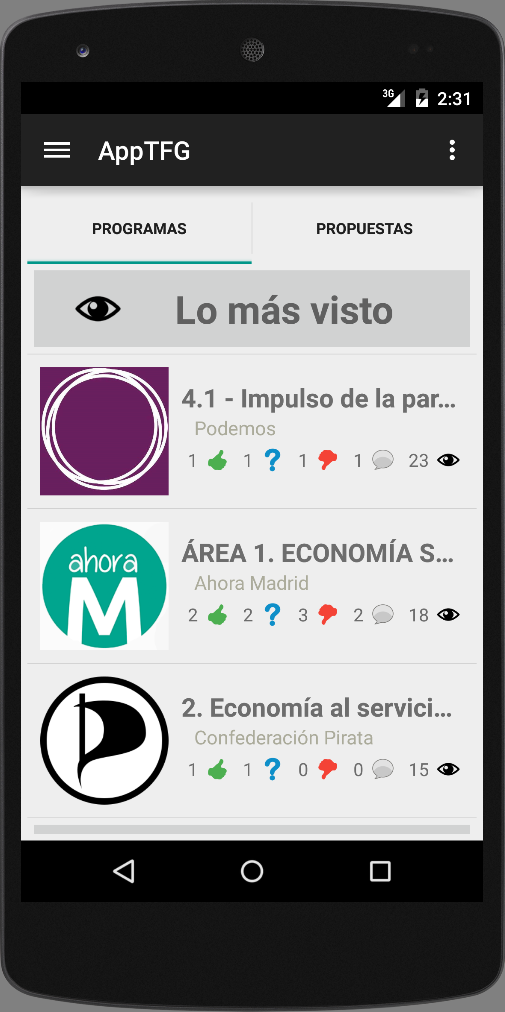
\includegraphics[keepaspectratio, scale=0.5]{Media/Captures/captTopSections.png}
\caption{Vista principal de secciones}
\label{fig:captTopSections}
\end{figure}

Dentro de cada sección podemos visualizar el contenido de la sección a la que referencia el programa, y tendremos la opción de valorarla de forma positiva o negativa. También añadimos la posibilidad de indicar que no se ha entendido la sección. Pues a la hora de leer una propuesta de gobierno ubicada en una sección del programa, bien nos puede gustar, disgustar o simplemente no haber entendido la idea y por ello no votarla de forma positiva o negativa.

\begin{figure}[H]
\centering
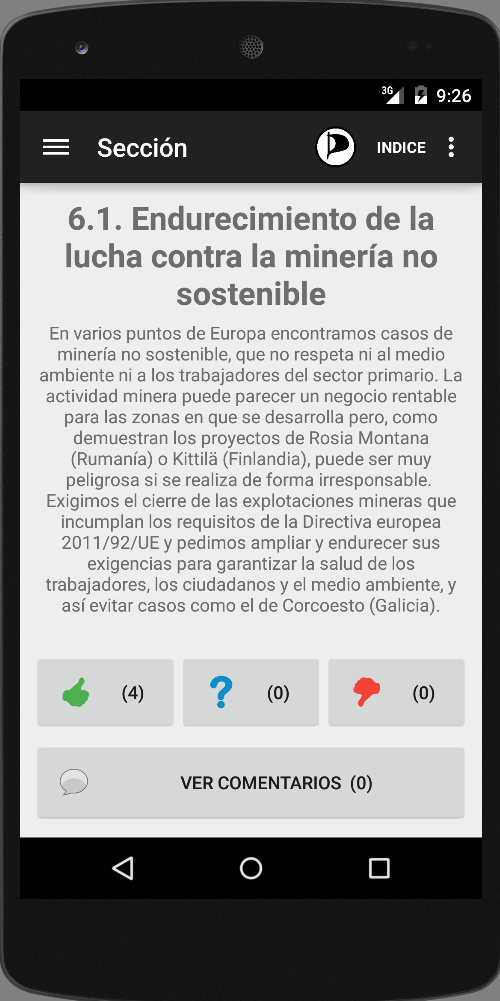
\includegraphics[keepaspectratio, scale=0.5]{Media/Captures/section.png}
\caption{Visualizando una sección}
\label{fig:captSection}
\end{figure}

Sin olvidarnos de la parte social, en cada sección podemos hacer comentarios para intentar debatir las ideas fundamentales que propone la sección. O incluso hacer referencia a una determinada frase o párrafo.
\subsection{Usabilidad}

\subsection{Revisión de la aplicación}
Una vez que habíamos implementado todos los objetivos fundamentales de la aplicación, decidimos hacer una revisión para poner a prueba la aplicación. Para ello nos reunimos con un grupo de Labodemo \cite{ref:labodemo}, responsables del desarrollo de los portales de participación ciudadana del partido político Podemos \cite{ref:podemos} y la candidatura ciudadana de unidad popular Ahora Madrid \cite{ref:ahoramadrid}.

\subsubsection{Reunión con Labodemo}
Tuvimos la oportunidad de establecer una conversación con dos miembros de Labodemo, en la que aprovechamos la oportunidad de mostrarles la aplicación que estábamos desarrollando. Ambos tenían experiencia en el desarrollo de plataformas de participación ciudadana en internet y nuevas tecnologías. Además fueron los responsables del desarrollo de los portales de participación del partido político Podemos y la candidatura ciudadana de unidad popular Ahora Madrid.

Limitarnos a mostrar las diferentes secciones de cada programa les resultó útil. Aunque no suficiente como para atraer a una cantidad considerable de usuarios. Antes de hablar con ellos, habíamos planteado desarrollar propuestas colaborativas en tiempo real aprovechando Wave. Pero no comprendieron la libertad de dar al usuarios la creación de propuestas colaborativas en tiempo real.

Dándole una vuelta al desarrollo de las propuestas de la aplicación, nos sugirieron que para atraer a usuarios a utilizar nuestra aplicación, deberíamos dejar cierta libertad a colectivos sociales. Por ejemplo, un grupo de animalistas debería tener un “espacio” en la aplicación donde poder crear sus propias propuestas, e incluso hacer comparativas personalizadas de lo que proponen los diferentes programas sobre los animales. Así surgirían propuestas y comparativas divididas por colectivos que abarcarían diferentes temáticas. Un usuario poco activo podría buscar un colectivo de profesores porque resulta ser su profesión, y ver las propuestas que se llevan a cabo o visualizar una comparativa respecto las medidas de educación de los diferentes programas políticos.

Organizar estas propuestas no sería tarea sencilla. En un principio se propuso como diferentes temas que puede tener un foro, en forma de post. Más tarde llegamos a la conclusión de que sería más cómodo para los colectivos dar la libertad de crear sus propios hilos, y en cada uno de ellos publicar las propuestas relacionadas con su colectivo.

Por último insistieron mucho en el tema de las comparativas. Sería de gran utilidad que la aplicación tuviera una parte de comparativas en la que los usuarios pudieran comparar los programas políticos en vez de leerlos sección por sección. Resultaría de gran interés a un autónomo visualizar las medidas que proponen los diferentes partidos políticos para los autónomos. Pero estas comparativas no podría realizarlas cualquiera, por lo que deberían realizarlas periodistas o expertos que hubieran realizado algún tipo de comparativa similar anteriormente. Nos sugirieron contactar con periodistas o colectivos que hubieran publicado algún tipo de comparativa en cuando a programas o medidas, para obtener algún tipo de ayuda o consejo a seguir.

\subsubsection{Conclusión}

La reunión con dos de los miembros de Labodemo resultó de gran interés. Pues desde que decidimos la idea que íbamos a implementar, nunca habíamos puesto en práctica la aplicación o al menos no la habíamos verificado con el “mundo real”.

Los integrantes de Labodemo eran expertos en desarrollo de portales de participación ciudadana. Y sobre todo estaban muy familiarizados con el uso común que les suele dar la gente a este tipo de aplicación. Por lo que sabían determinar las claves para que una aplicación tuviera un movimiento considerable de usuarios desde el comienzo.

El tema de visualizar los programas políticos no les gustó demasiado. Expusieron que un ciudadano de a pie, no iba a molestarse en leer los programas políticos. Bien porque no los entienda o porque les resulte aburridos. Ellos argumentaban que los colectivos sociales serían los usuarios más activos en nuestra aplicación, por lo que debíamos enfocar más el desarrollo hacia la partición ciudadana y el uso de propuestas o comparativas por colectivo.

Tras esta reunión decidimos replantear la aplicación en base a los consejos que obtuvimos con la reunión de Labodemo. Incluimos las propuestas como parte de nuestra aplicación y empezamos a pensar la forma de colaborar de grupos y colectivos. También intentamos contactar con colectivos y personas interesadas en el desarrollo de la aplicación. Finalmente, conseguimos concretar una entrevista con Javier de la Cueva \cite{ref:jdelacueva}.

\subsubsection{Reunión con Javier de la Cueva}

\subsubsection{Conclusión}